%%%%%%%%%%%%%%%%%%%%%%%%%%%%%%%%%%%%%%%%%%%%%%%%%%%%%%%%%%%%%%%%%%%%%%
% Article Unesp
%%%%%%%%%%%%%%%%%%%%%%%%%%%%%%%%%%%%%%%%%%%%%%%%%%%%%%%%%%%%%%%%%%%%%%
\documentclass[a4paper,times,12pt]{article}
\usepackage{amsthm}
\usepackage[figuresright]{rotating}
\usepackage{graphics}

\usepackage[utf8]{inputenc}
\usepackage[english]{babel}
\usepackage{graphicx}
\title{Métodos de Integração e Aplicações da Integral Definida}
\author{Victor Azadinho Miranda}
\date{\today}

\usepackage{amssymb}

\usepackage{graphicx}
\graphicspath{ {./images/} }

\usepackage{fancybox}
\usepackage{mathtools}
\usepackage{colortbl}
\usepackage{wasysym}
\usepackage{txfonts}
\usepackage{tikz}
%%%%%%%%%%%%%%%%%%%%%%%%%%%%%%%%%%%%%%%%%%%%%%%%%%%%%%%%%%%%%%%%%%%%%%%%
\begin{document}
\title{M\'{e}todos de Integraç\~{a}o e Aplicaç\~{o}es da Integral Definida}
\author{Victor Azadinho Miranda \\ Instituto de Bioci\^{e}ncias, Letras e Ci\^{e}ncias Exatas, Unesp - \\ Universidade Estadual Paulista (S\~{a}o Paulo State University) Rua Crist\'{o}v\~{a}o \\ Colombo 2265, Jd Nazareth, 15054-000, S\~{a}o Jos\'{e} do Rio Preto - SP, \\ Brazil. \quad e-mail: victor.azadinho@unesp.br}
\maketitle
%%%%%%%%%%%%%%%%%%%%%%%%%%%%%%%%%%%%%%%%%%%%%%%%%%%%%%%%%%%%%%%%%%%%%%%%
\section{Exerc\'{i}cios 7.4}
\hspace*{+15pt} 32) Calcular a integral indefinida.
\[ \int \frac{x}{\sqrt{x^{2}-1}}\tan^{3}{\sqrt{x^{2}-1}}dx \]
\begin{align*}
	u&=x^2-1 \\
	du&=2xdx
\end{align*}
\begin{gather*}
	=\int \frac{\tan ^3\left(\sqrt{u}\right)}{2\sqrt{u}}du \\
	=\frac{1}{2}\cdot \int \frac{\tan ^3\left(\sqrt{u}\right)}{\sqrt{u}}du
\end{gather*}
\begin{align*}
	v&=\sqrt{u} \\
	dv&=\frac{1}{2\sqrt{u}}du
\end{align*}
\begin{gather*}
	=\frac{1}{2}\cdot \int \:2\tan ^3\left(v\right)dv \\
	=\frac{1}{2}\cdot \:2\cdot \int \tan ^3\left(v\right)dv \\
	=\frac{1}{2}\cdot \:2\cdot \int \tan ^2\left(v\right)\tan \left(v\right)dv
\end{gather*}
\begin{align*}
	\tan ^2\left(x\right)&=-1+\sec ^2\left(x\right)
\end{align*}
\begin{gather*}
	=\frac{1}{2}\cdot \:2\cdot \int \left(-1+\sec ^2\left(v\right)\right)\tan \left(v\right)dv
\end{gather*}
\begin{align*}
	w&=\sec \left(v\right) \\
	dw&=\sec \left(x\right)\tan \left(x\right)dv
\end{align*}
\begin{gather*}
	=\frac{1}{2}\cdot \:2\cdot \int \frac{-1+w^2}{w}dw \\
	=\frac{1}{2}\cdot \:2\cdot \int \:-\frac{1}{w}+wdw \\
	=\frac{1}{2}\cdot \:2\left(-\int \frac{1}{w}dw+\int \:wdw\right) \\
	=\frac{1}{2}\cdot \:2\left(-\ln \left|w\right|+\frac{w^2}{2}\right)
\end{gather*}
\begin{align*}
	w&=\sec \left(v\right)
\end{align*}
\begin{gather*}
	=\frac{1}{2}\cdot \:2\left(-\ln \left|\sec \left(v\right)\right|+\frac{\sec \left(v\right)^2}{2}\right)
\end{gather*}
\begin{align*}
	v&=\sqrt{u}
\end{align*}
\begin{gather*}
	=\frac{1}{2}\cdot \:2\left(-\ln \left|\sec \left(\sqrt{u}\right)\right|+\frac{\sec \left(\sqrt{u}\right)^2}{2}\right)
\end{gather*}
\begin{align*}
	u&=x^2-1
\end{align*}
\begin{gather*}
	=\frac{1}{2}\cdot \:2\left(-\ln \left|\sec \left(\sqrt{x^2-1}\right)\right|+\frac{\sec ^2\left(\sqrt{x^2-1}\right)}{2}\right) \\
	=-\ln \left|\sec \left(\sqrt{x^2-1}\right)\right|+\frac{1}{2}\sec ^2\left(\sqrt{x^2-1}\right) \\
	=-\ln \left|\sec \left(\sqrt{x^2-1}\right)\right|+\frac{1}{2}\sec ^2\left(\sqrt{x^2-1}\right)+C
\end{gather*}
\newpage
\hspace*{+15pt} 70) Calcular a integral definida.
\[ \int _1^2\frac{dt}{t^4\sqrt{4+t^2}} \]
\begin{align*}
	t&=2\tan \left(u\right) \\
	dt&=2\sec ^2\left(u\right)
\end{align*}
\begin{gather*}
	=\int _{\arctan \left(\frac{1}{2}\right)}^{\frac{\pi }{4}}\frac{\sec \left(u\right)}{16\tan ^4\left(u\right)}du \\
	=\frac{1}{16}\cdot \int _{\arctan \left(\frac{1}{2}\right)}^{\frac{\pi }{4}}\frac{\sec \left(u\right)}{\tan ^4\left(u\right)}du
\end{gather*}
\begin{align*}
	v&=\tan \left(\frac{u}{2}\right) \\
	dv&=\sec ^2\left(\frac{u}{2}\right)
\end{align*}
\begin{gather*}
	=\frac{1}{16}\cdot \int _{\tan \left(\frac{\arctan \left(\frac{1}{2}\right)}{2}\right)}^{\sqrt{2}-1}\frac{\left(1-v^2\right)^3}{8v^4}dv \\
	=\frac{1}{16}\cdot \frac{1}{8}\cdot \int _{\tan \left(\frac{\arctan \left(\frac{1}{2}\right)}{2}\right)}^{\sqrt{2}-1}\frac{\left(1-v^2\right)^3}{v^4}dv \\
	=\frac{1}{16}\cdot \frac{1}{8}\cdot \int _{\tan \left(\frac{\arctan \left(\frac{1}{2}\right)}{2}\right)}^{\sqrt{2}-1}\frac{1}{v^4}-\frac{3}{v^2}+3-v^2dv \\
	=\frac{1}{16}\cdot\frac{1}{8}\left(\int_{\tan\left(\frac{\arctan\left(\frac{1}{2}\right)}{2}\right)}^{\sqrt{2}-1}\frac{1}{v^4}dv-\int_{\tan\left(\frac{\arctan\left(\frac{1}{2}\right)}{2}\right)}^{\sqrt{2}-1}\frac{3}{v^2}dv+\int_{\tan\left(\frac{\arctan\left(\frac{1}{2}\right)}{2}\right)}^{\sqrt{2}-1}3dv-\int_{\tan\left(\frac{\arctan\left(\frac{1}{2}\right)}{2}\right)}^{\sqrt{2}-1}v^2dv\right)
\end{gather*}
\begin{align*}
	\int _{\tan \left(\frac{\arctan \left(\frac{1}{2}\right)}{2}\right)}^{\sqrt{2}-1}\frac{1}{v^4}dv&=-\frac{1}{3\left(\sqrt{2}-1\right)^3}+\frac{1}{3\tan ^3\left(\frac{1}{2}\arctan \left(\frac{1}{2}\right)\right)} \\
	\int _{\tan \left(\frac{\arctan \left(\frac{1}{2}\right)}{2}\right)}^{\sqrt{2}-1}\frac{3}{v^2}dv&=3\left(-\sqrt{2}-1+\frac{1}{\tan \left(\frac{1}{2}\arctan \left(\frac{1}{2}\right)\right)}\right) \\
	\int _{\tan \left(\frac{\arctan \left(\frac{1}{2}\right)}{2}\right)}^{\sqrt{2}-1}3dv&=3\left(\sqrt{2}-1\right)-3\tan \left(\frac{\arctan \left(\frac{1}{2}\right)}{2}\right)\\
	\int _{\tan \left(\frac{\arctan \left(\frac{1}{2}\right)}{2}\right)}^{\sqrt{2}-1}v^2dv&=\frac{\left(\sqrt{2}-1\right)^3-\tan ^3\left(\frac{1}{2}\arctan \left(\frac{1}{2}\right)\right)}{3}
\end{align*}
\newpage
\rotatebox{90}{\(
	=\frac{1}{16}\cdot\frac{1}{8}\left(-\frac{1}{3\left(\sqrt{2}-1\right)^3}+\frac{1}{3\tan^3\left(\frac{1}{2}\arctan\left(\frac{1}{2}\right)\right)}-3\left(-\sqrt{2}-1+\frac{1}{\tan\left(\frac{1}{2}\arctan\left(\frac{1}{2}\right)\right)}\right)+3\left(\sqrt{2}-1\right)-3\tan\left(\frac{\arctan\left(\frac{1}{2}\right)}{2}\right)-\frac{\left(\sqrt{2}-1\right)^3-\tan^3\left(\frac{1}{2}\arctan\left(\frac{1}{2}\right)\right)}{3}\right)
\)}
\newpage
\section{Exerc\'{i}cios 7.9}
\hspace*{+15pt} 3) Calcular a integral indefinida.
\[ \int \frac{2dx}{sen\left(x\right)+tan\left(x\right)} \]
\begin{align*}
	u&=\tan \left(\frac{x}{2}\right) \\
	du&=\sec ^2\left(\frac{x}{2}\right)
\end{align*}
\begin{gather*}
	=2\cdot \int \:-\frac{\left(u+1\right)\left(u-1\right)}{2u}du \\
	=2\left(-\frac{1}{2}\cdot \int \frac{\left(u+1\right)\left(u-1\right)}{u}du\right) \\
	=2\left(-\frac{1}{2}\cdot \int \:u-\frac{1}{u}du\right) \\
	=2\left(-\frac{1}{2}\left(\int \:udu-\int \frac{1}{u}du\right)\right)
\end{gather*}
\begin{align*}
	\int \:udu&=\frac{u^2}{2} \\
	\int \frac{1}{u}du&=\ln \left|u\right|
\end{align*}
\begin{gather*}
	=2\left(-\frac{1}{2}\left(\frac{u^2}{2}-\ln \left|u\right|\right)\right)
\end{gather*}
\begin{align*}
	u=\tan \left(\frac{x}{2}\right)
\end{align*}
\begin{gather*}
	=2\left(-\frac{1}{2}\left(\frac{\tan ^2\left(\frac{x}{2}\right)}{2}-\ln \left|\tan \left(\frac{x}{2}\right)\right|\right)\right) \\
	=-\frac{1}{2}\tan ^2\left(\frac{x}{2}\right)+\ln \left|\tan \left(\frac{x}{2}\right)\right| \\
	=-\frac{1}{2}\tan ^2\left(\frac{x}{2}\right)+\ln \left|\tan \left(\frac{x}{2}\right)\right|+C
\end{gather*}
\newpage
\section{Exerc\'{i}cios 8.4}
\hspace*{+15pt} 7) Encontrar o comprimento de arco da curva dada.
\[ y=\frac{1}{2}\left(e^{x}+e^{-x}\right)\text{, de }\left(0,1\right)\text{ a }\left(1,\frac{e+e^-1}{2}\right) \]
\\
\par Primeiro montamos o sistema:
\[
	\begin{cases}
		x&=t \\
		y&=\frac{1}{2}\left(e^{t}+e^{-t}\right)
	\end{cases}
	,t\in[0,1]
\]
\par Então calculamos as derivadas:
\begin{align*}
	t'\:&=1 \\
	\left(\frac{1}{2}\left(e^t+e^{-t}\right)\right)'\:&=\frac{1}{2}\left(e^t-e^{-t}\right)
\end{align*}
\par Por fim aplicamos a fórmula:
\[
	s=\int_{t_0}^{t_1}\sqrt{[x'(t)]^2+[y'(t)]^2}dt
\]
\begin{gather*}
	s = \int_0^1\sqrt{[1]^2+[\frac{1}{2}(e^x+e^{-x})]^2}dt \\
	=\int_0^1\sqrt{1+\left(\frac{1}{2}\left(e^t+e^{-t}\right)\right)^2}dt \\
	=\int_0^1\sqrt{1+\frac{\left(e^t+e^{-t}\right)^2}{4}}dt \\
	=\int_0^1\sqrt{\frac{e^{-2t}+e^{2t}+6}{4}}dt \\
	=\int_0^1\frac{\sqrt{e^{-2t}+e^{2t}+6}}{\sqrt{4}}dt \\
	=\int_0^1\frac{\sqrt{e^{-2t}+e^{2t}+6}}{2}dt
\end{gather*}
\newpage
\section{Exerc\'{i}cios 8.7}
\hspace*{+15pt} 8) Determinar o volume do sólido de revolução gerado pela rotação, em torno do eixo dos \( y \) da região \( R \) delimitada pelos gráficos da equação dada.
\[ x=y^2+1,x=\frac{1}{2},y=-2\text{ e }y=2 \]
\\
\par Primeiro definimos \(f(y)\):
\begin{gather*}
	\begin{cases}
		x&=y^2+1 \\
		x&=\frac{1}{2}
	\end{cases} \\
	\frac{1}{2}=y^2+1 \\
	y^2+\frac{1}{2}=0 \\
	f(y)=y^2+\frac{1}{2}
\end{gather*}
\par Então aplicamos a fórmula:
\[
	V=\pi\int_a^b[f(y)]^2dy
\]
\begin{align*}
	a&=-2 \\
	b&=2
\end{align*}
\begin{gather*}
	V=\pi \int_{-2}^2[y^2+\frac{1}{2}]^2dy \\
	=\pi \int _{-2}^2y^4+y^2+\frac{1}{4}dy \\
	=\pi \int _{-2}^2y^4dy+\int _{-2}^2y^2dy+\int _{-2}^2\frac{1}{4}dy
\end{gather*}
\begin{align*}
	\int _{-2}^2y^4dy&=\frac{64}{5} \\
	\int _{-2}^2y^2dy&=\frac{16}{3} \\
	\int _{-2}^2\frac{1}{4}dy&=1
\end{align*}
\begin{gather*}
	=\pi \frac{64}{5}+\frac{16}{3}+1 \\
	=\pi \frac{287}{15} \\
	=\frac{287\pi }{15} \\
	\approx 60.10913\dots 
\end{gather*}
\newpage
\section{Exerc\'{i}cios 8.11}
\hspace*{+15pt} 15) Esboçar o gráfico da curva dada em coordenada polar.
\[
	r=2-\cos\theta
\]
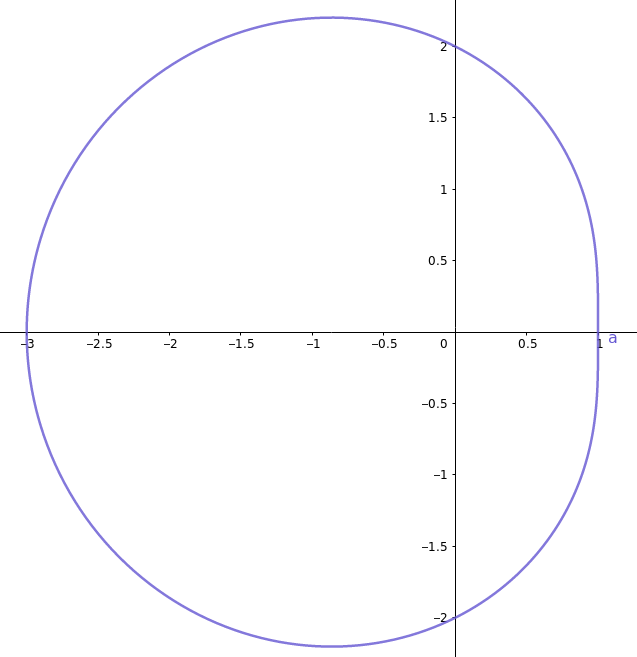
\includegraphics[width=\textwidth]{8-11-15}
\newpage
\hspace*{+15pt} 51) Calcular a área limitada pela curva dada.
\[
	r=3\sin2\theta
\]
\par Analisando o gráfico abaixo podemos notar que o gráfico dessa função é simétrico.
\\
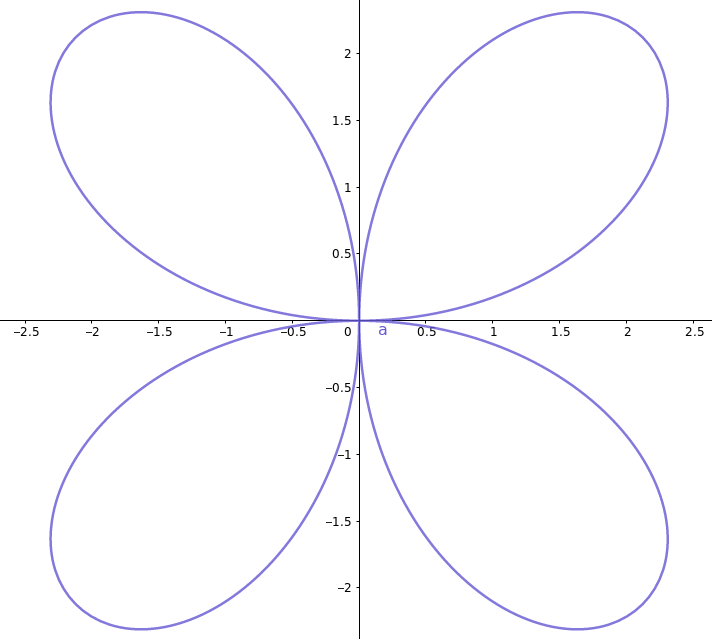
\includegraphics[width=\textwidth]{8-11-51}
\\
\par Portanto, para descobrir a área, basta calcular no primeiro quadrante e multiplicar por quatro. Aplica-se, então, a seguinte fórmula.
\[
	A=\frac{1}{2}\int_\alpha^\beta[f\left(\theta\right)]^2d\theta
\]
\begin{align*}
	\alpha&=0 \\
	\beta&=\frac{\pi}{2}
\end{align*}
\begin{gather*}
	\frac{1}{2}\cdot \int _0^{\frac{\pi }{2}}\left(3\sin \left(2\theta\right)\right)^2d\theta \\
	=\frac{1}{2}\cdot \int _0^{\frac{\pi }{2}}9\sin ^2\left(2\theta\right)d\theta \\
	=\frac{1}{2}\cdot 9\cdot \int _0^{\frac{\pi }{2}}\sin ^2\left(2\theta\right)d\theta
\end{gather*}
\begin{align*}
	\sin ^2\left(x\right)=\frac{1-\cos \left(2x\right)}{2}
\end{align*}
\begin{gather*}
	=\frac{1}{2}\cdot 9\cdot \int _0^{\frac{\pi }{2}}\frac{1-\cos \left(2\cdot \:2\theta\right)}{2}d\theta \\
	=\frac{1}{2}\cdot 9\cdot \int _0^{\frac{\pi }{2}}\frac{1}{2}\left(1-\cos \left(4\theta\right)\right)d\theta \\
	=\frac{1}{2}\cdot 9\cdot \frac{1}{2}\cdot \int _0^{\frac{\pi }{2}}1-\cos \left(4\theta\right)d\theta \\
	=\frac{1}{2}\cdot 9\cdot \frac{1}{2}\left(\int _0^{\frac{\pi }{2}}1d\theta-\int _0^{\frac{\pi }{2}}\cos \left(4\theta\right)d\theta\right)
\end{gather*}
\begin{align*}
	\int _0^{\frac{\pi }{2}}1d\theta&=\frac{\pi }{2} \\
	\int _0^{\frac{\pi }{2}}\cos \left(4\theta\right)d\theta&=0
\end{align*}
\begin{gather*}
	=\frac{1}{2}\cdot 9\cdot \frac{1}{2}\left(\frac{\pi }{2}-0\right)
	=\frac{1}{2}\cdot \frac{9\pi }{4} \\
	=\frac{9\pi }{8} \\
	\approx 3.53429\dots
\end{gather*}
\par Por fim, multiplicamos o resultado por quatro.
\begin{gather*}
	4\cdot \frac{9\pi }{8} \\
	=\frac{9\pi }{2} \\
	\approx 14.13716\dots
\end{gather*}
\end{document}